\documentclass{beamer}
\usecolortheme[named=brown]{structure}
\usetheme{Malmoe}
\usepackage{natbib}
\usepackage{graphicx}

\author{James Church}
\title{A Gentle Introduction to R}

\begin{document}

\frame[plain]{ \titlepage }

\begin{frame}{A Gentle Introduction to R}

    Outline

    \begin{itemize}
        \item Why R?
        \item Tools that I'm using in this presentation.
        \item Important Data Types
        \item The Basics
        \item Random Number Generation
        \item Computing Pi
        \item Data Analysis with Data Frames
        \item Simple Linear Regression
        \item Multiple Linear Regression
    \end{itemize}

\end{frame}

\section{Introduction}

\subsection{Why?}

\begin{frame}{Why R?}
     \begin{itemize}
        \item You wish to analyze.
        \item You wish to create beautiful plots.
    \end{itemize}
\end{frame}

\subsection{The Goods}

\begin{frame}{Tools Used in this Presentation}
    \begin{itemize}
        \item R
        \item RStudio
    \end{itemize}
\end{frame}

\subsection{Basic Storage}

\begin{frame}{Data Types}

     The (IMO) Important Data Types

     \begin{itemize}
        \item Numerical
        \item Character
        \item Logical (TRUE, T, FALSE, F)
        \item Vectors
        \item Data Frames
        \item Factors
    \end{itemize}
\end{frame}

\subsection{Do or do not.}

\begin{frame}[fragile]{Getting Started}

Which of the three statements is the correct way to assign a variable in R?

\begin{verbatim}
> a <- 1
> 2 -> b
> c = 3
\end{verbatim}

Answer: All three. The ``R way''\texttrademark of assigning variables is to use the left arrow.

\end{frame}

\begin{frame}[fragile]{Vectors :: 1}

Like arrays, but better.

\begin{verbatim}
> my.vector <- c(1, 3, 7, 15, 31)
> my.vector + 1
[1]  2  4  8 16 32
> my.vector * 2
[1]  2  6 14 30 62
> my.vector ^ 2
[1]   1   9  49 225 961
> my.vector > 10
[1] FALSE FALSE FALSE  TRUE  TRUE
\end{verbatim}

\end{frame}

\begin{frame}[fragile]{Vectors :: 2}

Like arrays, but better.

\begin{verbatim}
> my.vector <- c(1, 3, 7, 15, 31)
> sum(my.vector)
[1] 57
> sum(my.vector>10)
[1] 2
> mean(my.vector)
[1] 11.4
> median(my.vector)
[1] 7
> sd(my.vector)
[1] 12.19836
\end{verbatim}

\end{frame}

\section{Random Numbers}

\subsection{Basics}

\begin{frame}[fragile]{Random Numbers}
    \begin{itemize}
        \item Normal: rnorm(n, mean=0, sd=1)
        \item Uniform: runif(n, low=0, high=1)
    \end{itemize}
\end{frame}

\subsection{Quick Test: Normal}
\begin{frame}[fragile]{Quick Test for Normal}

Is it true that `rnorm' produces a normal curve with a mean of 0 and a standard deviation of 1?

\begin{verbatim}
> v <- rnorm(1000)
> mean(v)
[1] 0.06681055
> sd(v)
[1] 0.9872857
> plot(v)
> hist(v)
\end{verbatim}

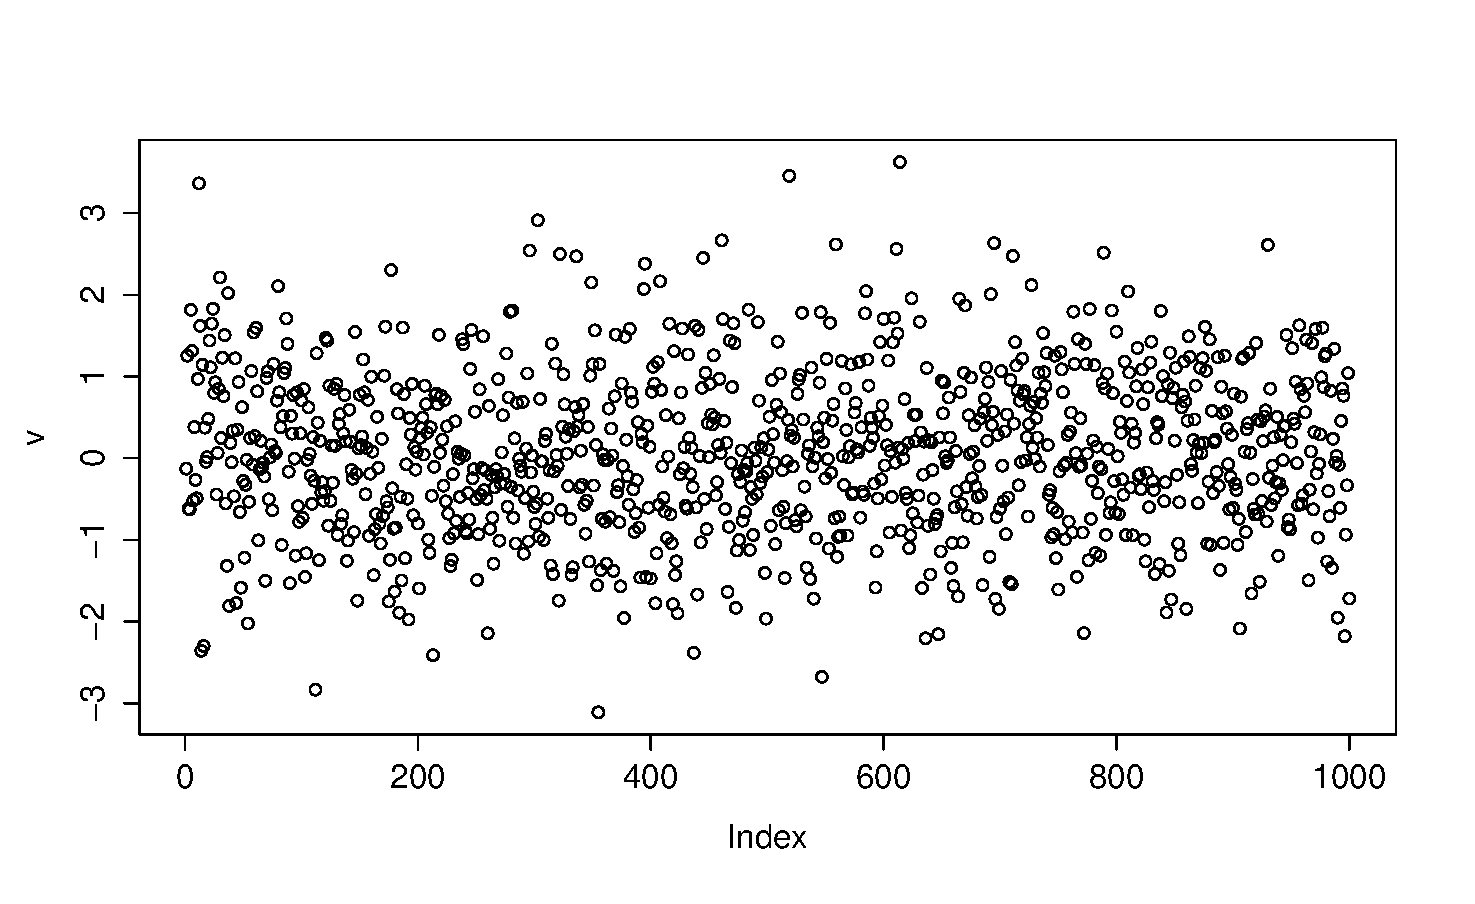
\includegraphics[scale=0.2]{normal_plot.eps}
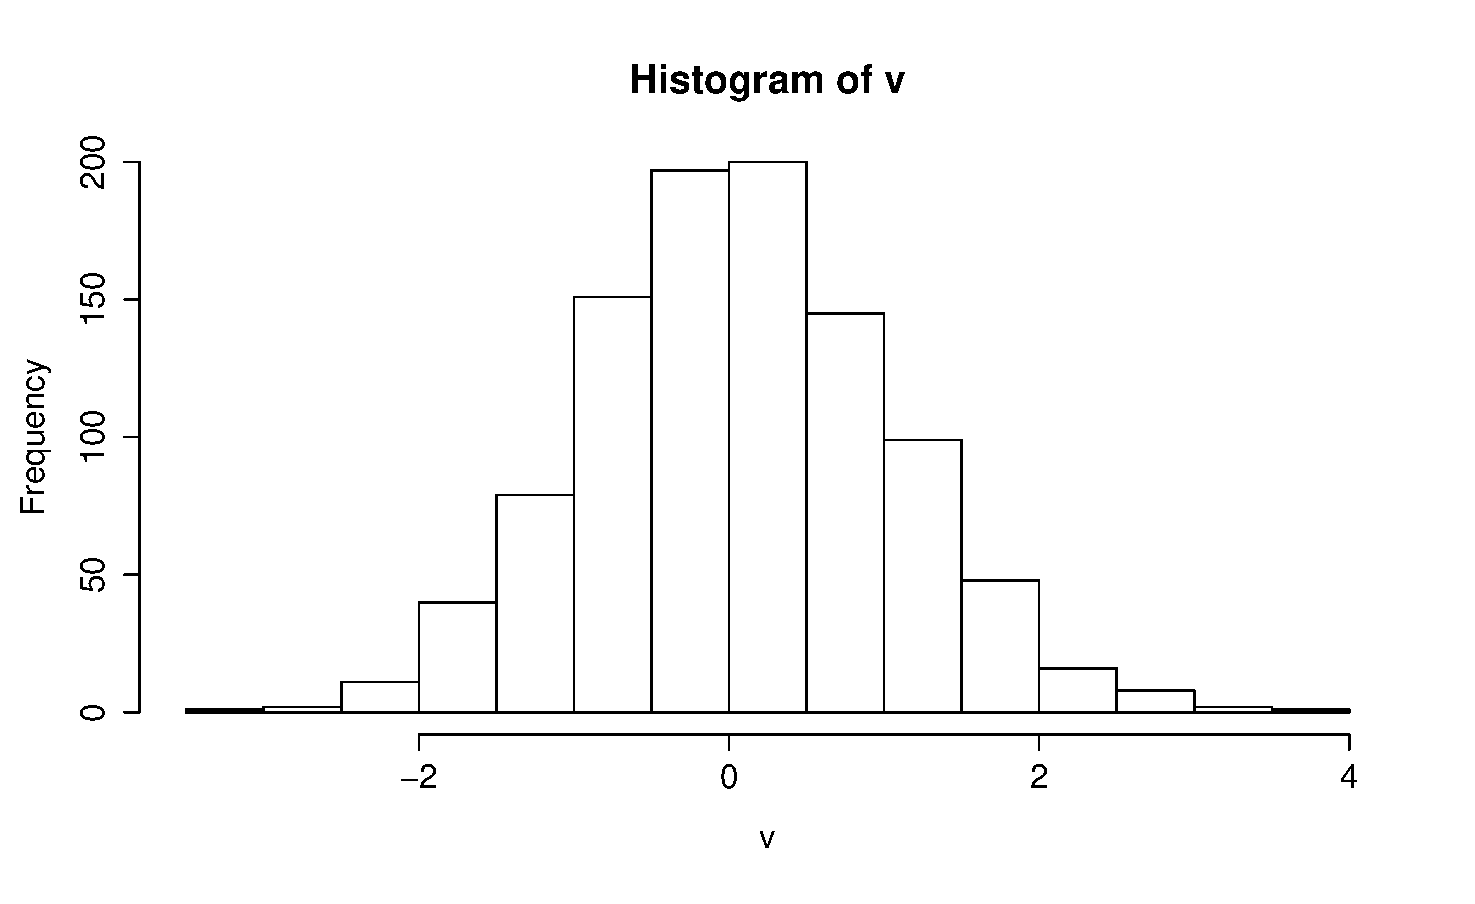
\includegraphics[scale=0.2]{normal_hist.eps}

\end{frame}

\subsection{Quick Test: Uniform}
\begin{frame}[fragile]{Quick Test for Uniform}

Is it true that `runif' produces a uniform curve with a low of 0 and a high of 1?

\begin{verbatim}
> v <- runif(1000)
> min(v)
[1] 0.0007571692
> max(v)
[1] 0.9999074
> plot(v)
> hist(v)
\end{verbatim}

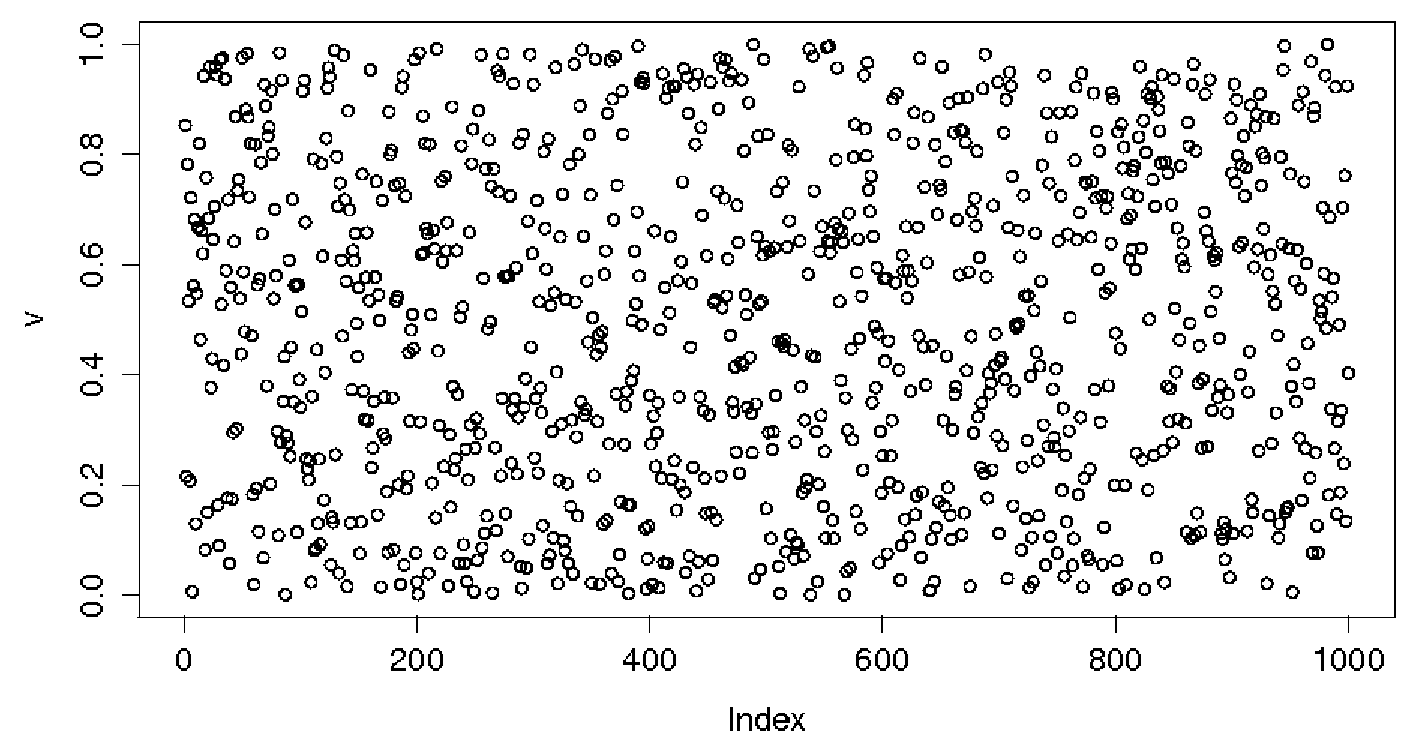
\includegraphics[scale=0.2]{uniform_plot.eps}
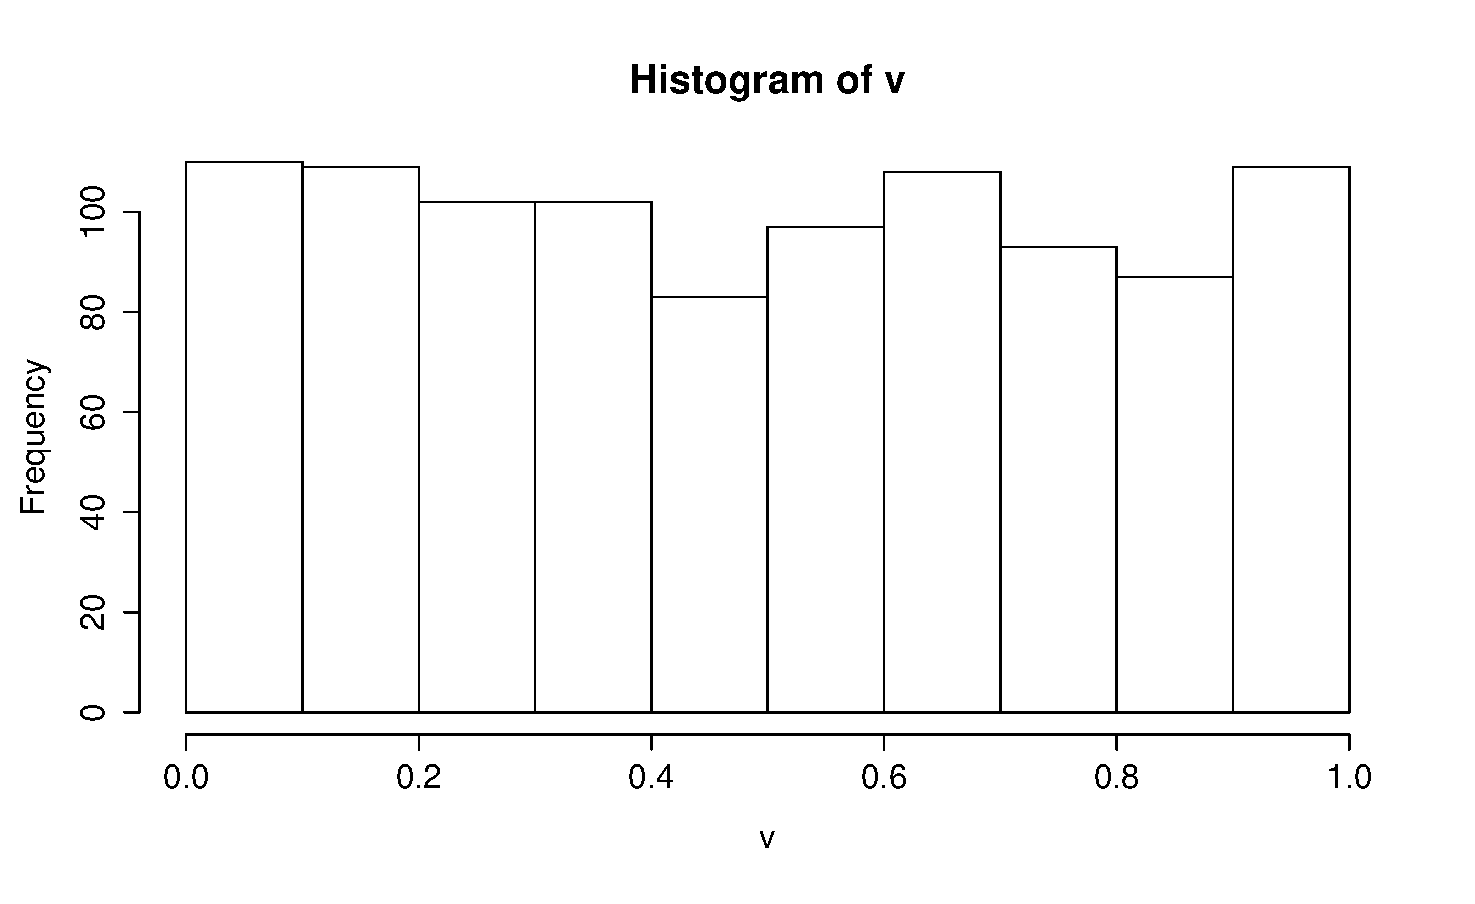
\includegraphics[scale=0.2]{uniform_hist.eps}

\end{frame}

\subsection{Basics}

\section{Computing Pi}

\subsection{Theory}

\begin{frame}{Computing Pi using Random Numbers :: Theory}

\begin{itemize}
    \item A square with sides of length 2 has its center at the origin.
    \item A circle with a radius of length 1 has its center at the origin.
    \item The length of the side of the square is 2 times the radius of the circle. 
\item Area of the square: $(2r)^2$ or $4r^2$ or $4$.
\item Area of the circle: $\pi r^2$ or $\pi$.

\item The ratio of the area of the two shapes is

\begin{math}
\frac{\pi}{4} = \frac{Area\:of\:the\:Circle}{Area\:of\:the\:Square}
\end{math}

\item This means we can write $\pi$ as

\begin{math}
\pi = \frac{4 \times Area\:of\:the\:Circle}{Area\:of\:the\:Square}
\end{math}

\end{itemize}
\end{frame}

\subsection{Practice}

\begin{frame}{Computing Pi using Random Numbers :: Practice}

\begin{itemize}
\item Imagine our square is now a dartboard.
\item We have 100,000 darts to throw at the dartboard.
\item All 100,000 darts must land in the square.
\item We count the darts landing in the circle.
\item We then compute $\pi$:

\begin{math}
\pi = \frac{4 \times Area\:of\:the\:Circle}{Area\:of\:the\:Square} = \frac{4 \times Darts\:in\:the\:Circle}{100,000}
\end{math}

\end{itemize}
\end{frame}

\subsection{Code}

\begin{frame}[fragile]{Computing Pi using Random Numbers :: Code}

\begin{verbatim}
> # Start throwing darts
> n <- 100000
> x <- runif(n, -1, 1)
> y <- runif(n, -1, 1)
\end{verbatim}

\begin{verbatim}
> # Determine which darts are in the circle
> in.circle <- sqrt(x^2 + y^2)<=1
\end{verbatim}

\begin{verbatim}
> # Estimate pi and calcualte the error.
> estimated.pi <- 4 * sum(in.circle) / n
> estimated.pi
[1] 3.14512
> estimated.pi.error <- 100*abs(estimated.pi - pi)/pi
> estimated.pi.error
[1] 0.1122789
\end{verbatim}

\end{frame}

\subsection{Plotting}

\begin{frame}[fragile]{Computing Pi using Random Numbers :: Plotting}

\begin{verbatim}
> matplot(x[in.circle==T], y[in.circle==T],
          col='blue');
> matplot(x[in.circle==F], y[in.circle==F],
          col='red', add=T)
\end{verbatim}

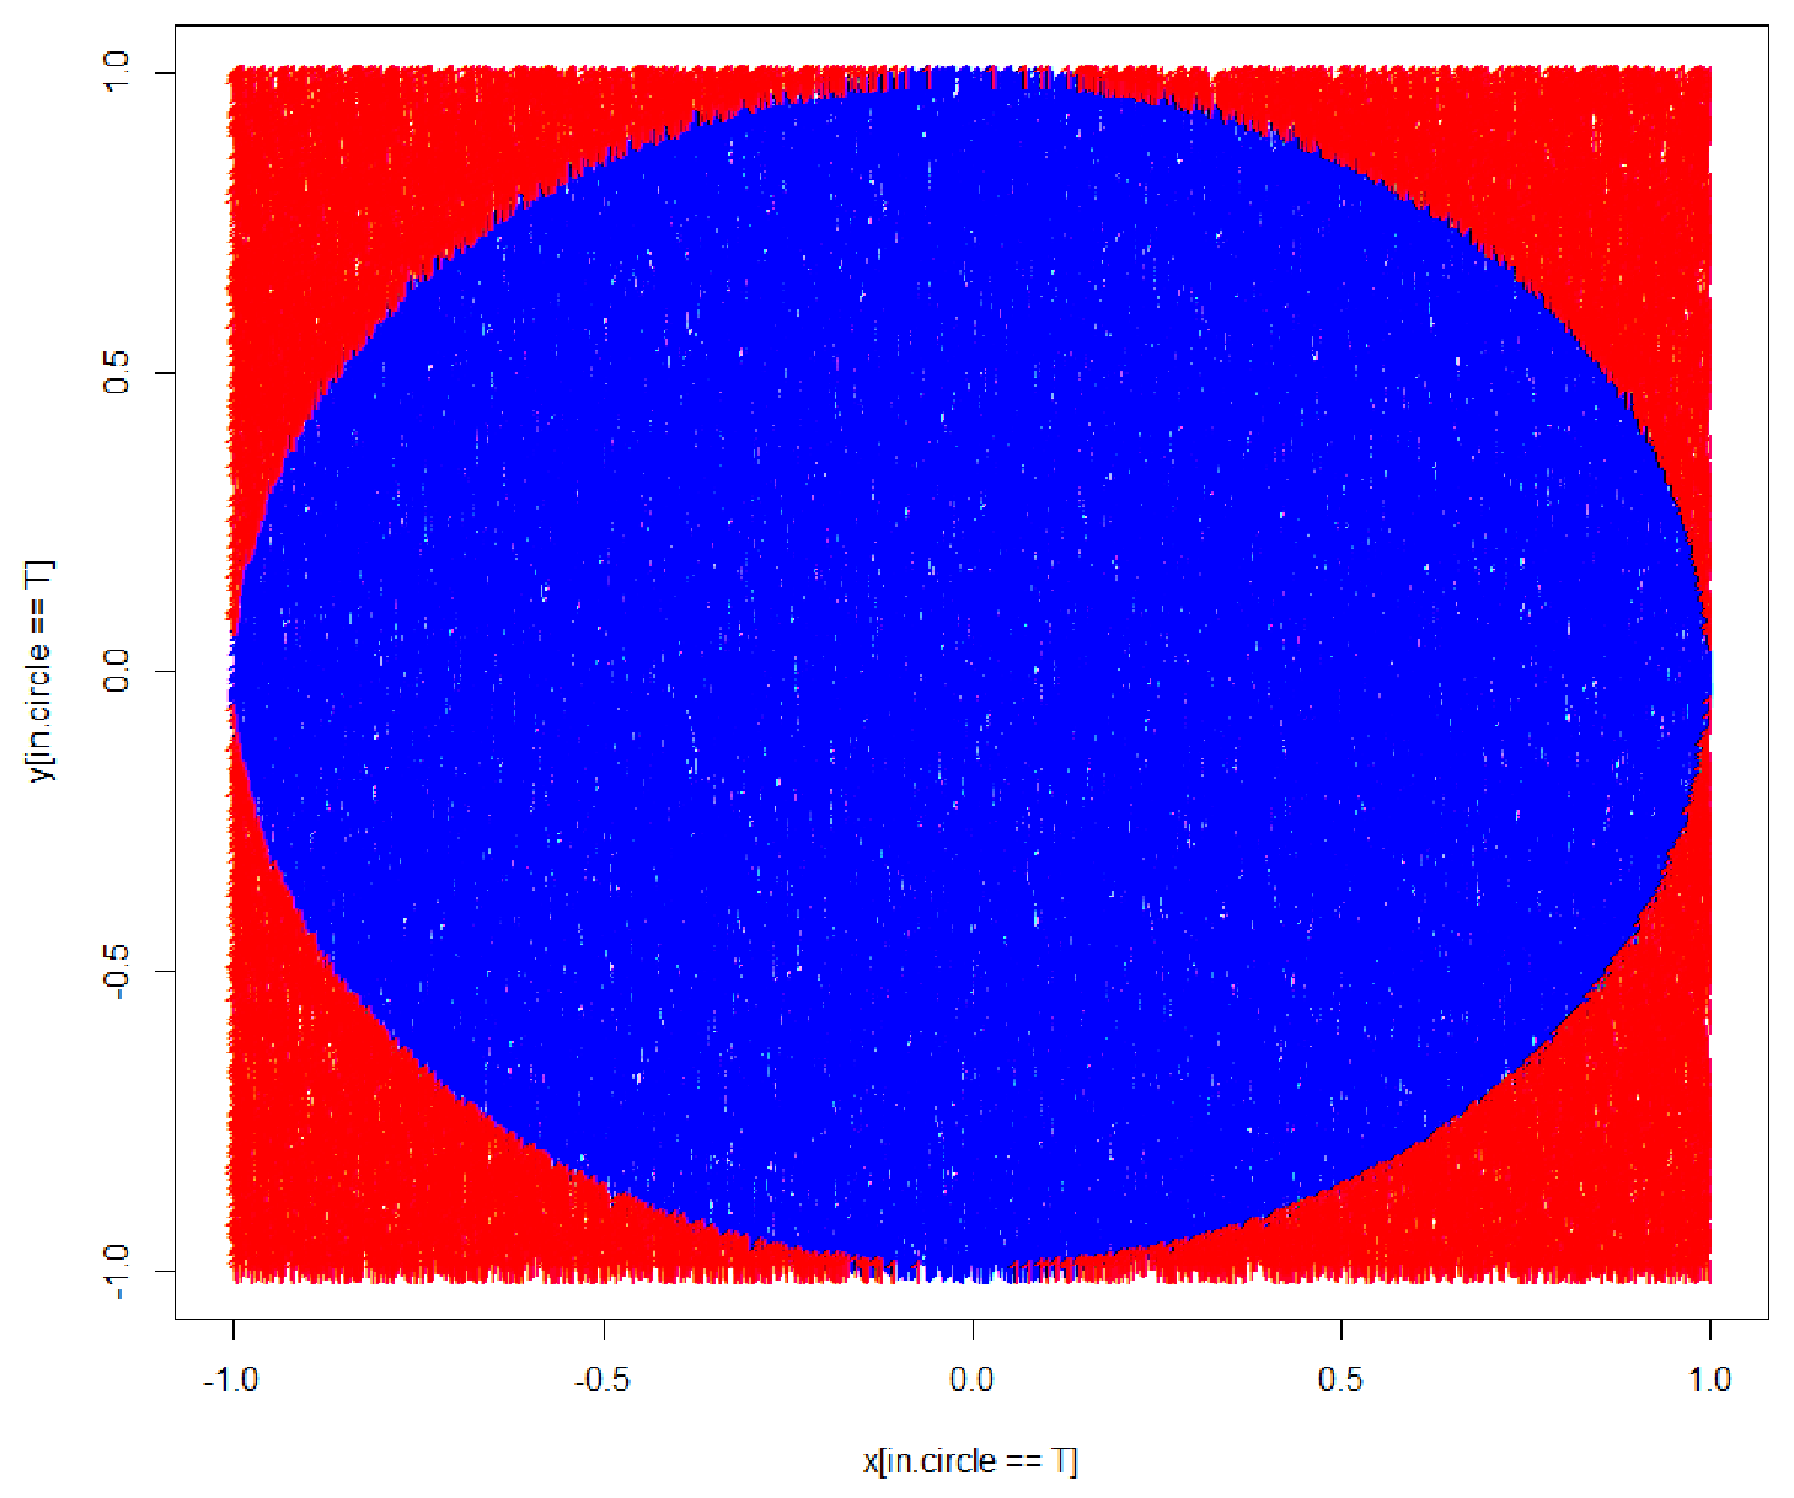
\includegraphics[scale=0.19]{dartboard.eps}

\end{frame}

\section{Data Analysis with Data Frames}

\subsection{Reading a CSV file}

\begin{frame}[fragile]{Data Analysis :: Reading CSV Files}

\begin{verbatim}
> setwd("~/code/RIntro") # Your working directory
> tax <- read.csv('Tax_Year_2007_County_Income_Data.csv')
> summary(tax)
     Wages              Dividend           Interest       
 Min.   :       -1   Min.   :      -1   Min.   :      -1  
 1st Qu.:   125193   1st Qu.:    2434   1st Qu.:    6200  
 Median :   320627   Median :    7234   Median :   14626  
 Mean   :  3327009   Mean   :   98482   Mean   :  155972  
 3rd Qu.:   999196   3rd Qu.:   25503   3rd Qu.:   41676  
 Max.   :669494988   Max.   :19742493   Max.   :34132623
> names(tax)
 [1] "State.Code"      "County.Code"     "State.Abbr"
     "County"          "Num.Tax.Returns" "Num.Exemptions"
     "Adjusted.Gross" 
 [8] "Wages"           "Dividend"        "Interest"       
\end{verbatim}

\end{frame}

\subsection{Income versus Number of Exemptions}

\begin{frame}[fragile]{Data Analysis :: Preparing Our Data}
Does wealth influence the number of exemptions?

\begin{footnotesize}
\begin{verbatim}
> tax$Adjusted.Gross.Per.Return <- tax$Adjusted.Gross / tax$Num.Tax.Returns
> tax$Exemption.Per.Return <- tax$Num.Exemptions / tax$Num.Tax.Returns
> median(tax$Adjusted.Gross.Per.Return)
[1] 40.77554
> median(tax$Exemption.Per.Return)
[1] 2.066597
> plot(tax$Adjusted.Gross.Per.Return, tax$Exemption.Per.Return)
\end{verbatim}
\end{footnotesize}

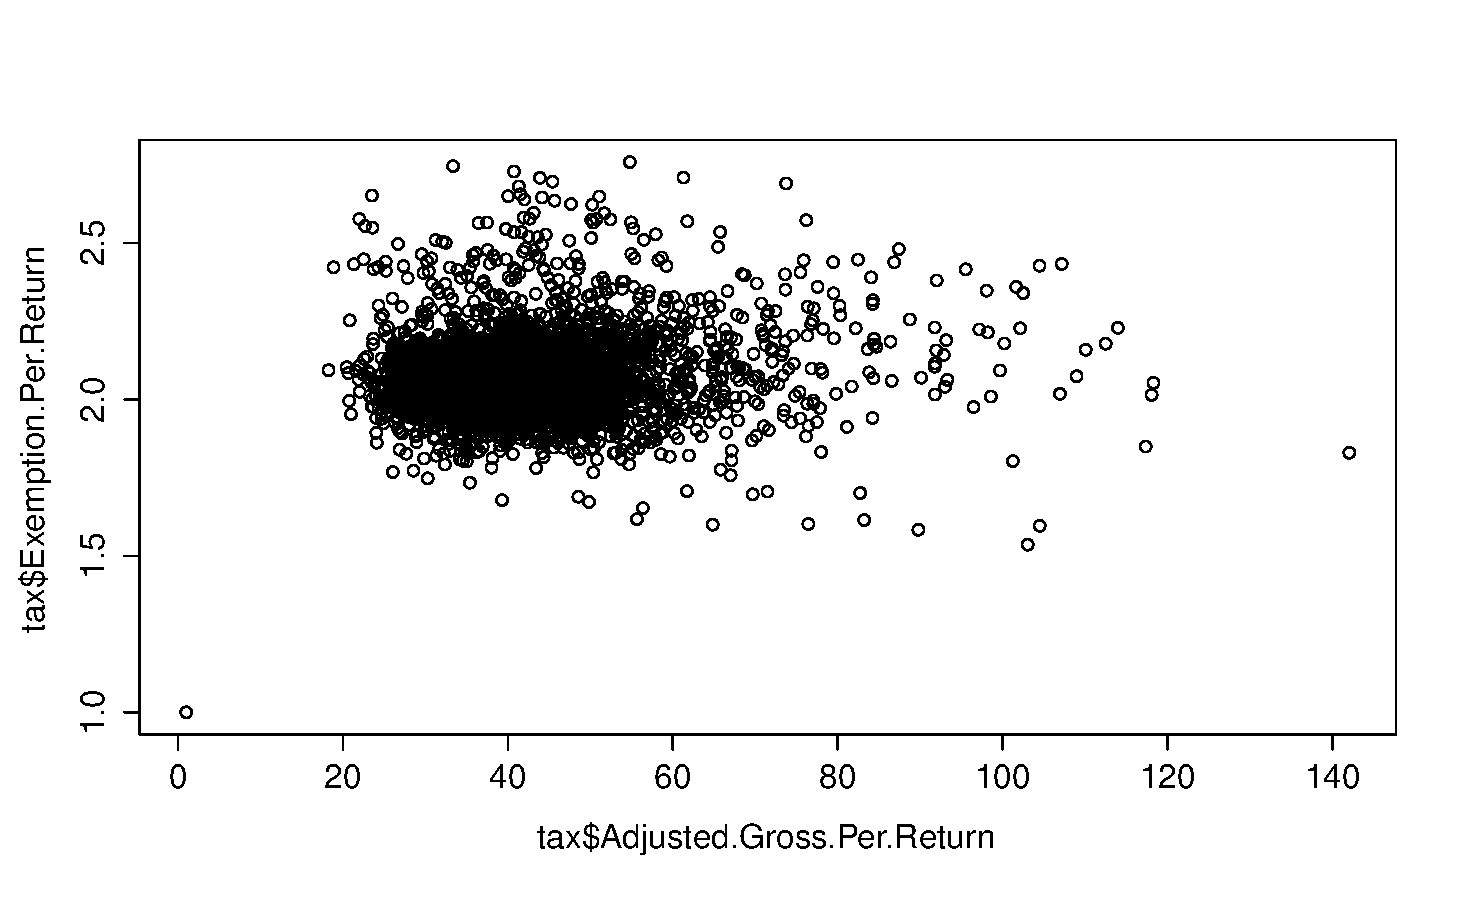
\includegraphics[scale=0.2]{income_v_exemptions.eps}

\end{frame}

\subsection{Statistical Analysis with lm}

\begin{frame}[fragile]{Data Analysis :: Performing the Test}
Does the number of exemptions \textbf{depend} on the adjusted gross income?

\begin{footnotesize}
\begin{verbatim}
> summary(lm(tax$Exemption.Per.Return ~ tax$Adjusted.Gross.Per.Return))
Coefficients:
                               Estimate Std. Error t value Pr(>|t|)    
(Intercept)                   2.0408565  0.0084952 240.237  < 2e-16 ***
tax$Adjusted.Gross.Per.Return 0.0008869  0.0001891   4.691 2.83e-06 ***
---
Signif. codes:  0 ‘***’ 0.001 ‘**’ 0.01 ‘*’ 0.05 ‘.’ 0.1 ‘ ’ 1 

Residual standard error: 0.1372 on 3191 degrees of freedom
Multiple R-squared: 0.006849,   Adjusted R-squared: 0.006538 
F-statistic: 22.01 on 1 and 3191 DF,  p-value: 2.832e-06
\end{verbatim}
\end{footnotesize}

\end{frame}

\begin{frame}[fragile]{Data Analysis :: Preparing Our Data}
Does wealth influence the number of exemptions in Mississippi?

\begin{footnotesize}
\begin{verbatim}
> plot(tax$Adjusted.Gross.Per.Return[tax$State.Abbr=="MS"],
       tax$Exemption.Per.Return[tax$State.Abbr=="MS"])
\end{verbatim}
\end{footnotesize}

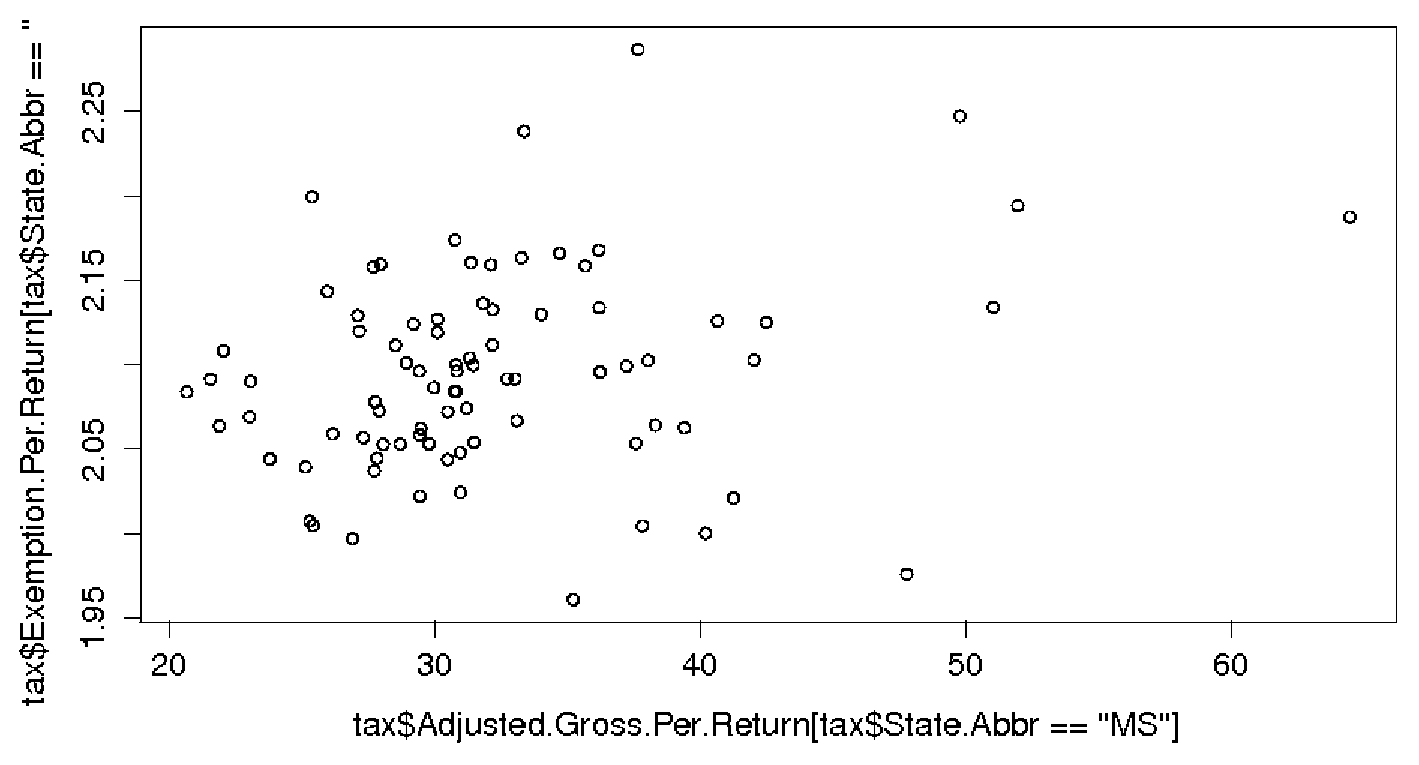
\includegraphics[scale=0.2]{income_v_exemptions_ms.eps}

\end{frame}

\begin{frame}[fragile]{Data Analysis :: Performing the Test}
Does the number of exemptions \textbf{depend} on the adjusted gross income in Mississippi?

\begin{footnotesize}
\begin{verbatim}
> summary(lm(tax$Exemption.Per.Return[tax$State.Abbr=="MS"] ~
             tax$Adjusted.Gross.Per.Return[tax$State.Abbr=="MS"]))

Coefficients:
             Estimate Std. Error t value Pr(>|t|)    
(Intercept) 2.0261054  0.0291375  69.536   <2e-16 ***
tax$Adj...  0.0021531  0.0008805   2.445   0.0166 *  
---
Signif. codes:  0 ‘***’ 0.001 ‘**’ 0.01 ‘*’ 0.05 ‘.’ 0.1 ‘ ’ 1 

Residual standard error: 0.05834 on 81 degrees of freedom
Multiple R-squared: 0.06875,    Adjusted R-squared: 0.05725 
F-statistic: 5.979 on 1 and 81 DF,  p-value: 0.01664
\end{verbatim}
\end{footnotesize}

\end{frame}

\end{document}
